\documentclass[10pt]{article}
\usepackage{fontspec}
\usepackage{polyglossia}
\setdefaultlanguage{french}
\usepackage[a4paper,margin=2.5cm]{geometry}
\usepackage{circuitikz}
\usepackage{url,hyperref}
\usepackage{siunitx}
\usepackage{schemabloc}
\usepackage{listings}
\usepackage{auto-pst-pdf}
\usepackage{pst-circ}
\usepackage{soul}
\usepackage{verbatim}
\usepackage{lmodern}
\usepackage{tikz}
\usepackage{xunicode,xltxtra}
\usepackage{graphicx}
\usepackage{amsmath}
\usepackage{minted}
\usepackage{multicol}
\title{
\includegraphics{inp-enseeiht} \\ ~ \\ ~ \\ ~ \\ ~ \\ BE Jonction PN}
\author{Ken Hasselmann, Guilhem Saurel}
\date{\oldstylenums{\today}}
\begin{document}

 \begin{titlepage}
  \maketitle
  \tableofcontents
 \end{titlepage}

 \section{Évaluation des caractéristiques principales. Jonction à l'équilibre}
  \subsection{A quel potentiel doit-on relier le substrat ? Pourquoi ?}
   Afin de ne pas perturber la partie $P^+N$ de la diode, il faut polariser la diode NP (du substrat) en inverse. Pour cela, il faut donc relier le substrat à la masse.

  \subsection{Calculer le potentiel de diffusion de la diode.}
   $\Phi_{NP} = U_T \ln\cfrac{N_A N_D}{n_i^2}$.
   
   AN : $\Phi_{NP} = 0.8V$.

  \subsection{Calculer la largeur de la zone de charge d’espace globale et dans chacune des 2 régions. Justifier. En déduire la largeur électrique de chacune des régions.} 
   La largeur de la zone de charge d'espace globale vaut $\delta = \sqrt{\cfrac{2\varepsilon}{qN^\ast}\Phi_{NP}}$ où $N^\ast = \cfrac{N_A N_D}{N_A + N_D} \simeq \min(N_A,N_D)$. 
   
   AN : $\delta = 5.78\cdot 10^{-5}cm$

   On en déduit la largeur de la zone de charge d'espace de chacune des régions grâce aux formules $N_A \delta_p = N_D \delta_n$ et $\delta = \delta_p + \delta_n$, donc, en exprimant $\delta_p$ dans les deux formules, on obtient $\delta_p = \cfrac{N_D}{N_A}\delta_n = \delta - \delta_n \Rightarrow \delta_n =\cfrac{\delta}{\cfrac{N_D}{N_A} +1}$ \& $\delta_p = \delta - \delta_n$

   AN : $\delta_n = 5.77\cdot 10^{-5} cm$ \& $\delta_p = 8.66\cdot 10^{-8}cm$

   On en déduit la largeur électrique grâce à la formule $W = X - \delta$

   AN : $W_n = 2.42\cdot 10^{-4}cm$ \& $W_p = 9.91\cdot 10^{-6}cm$

  \subsection{Calculer le courant de saturation de la diode sachant que dans le silicium en faible niveau d’injection, la durée de vie des porteurs est de $1\mu s$ pour un dopage de $10^{16} cm^{-3}$.}
   La formule de base pour le calcul du courant de saturation de la diode est 
   
   $I_s = q A_j n_i^2 \left[\cfrac{D_N}{N_A L_n \tanh\cfrac{W_P}{L_n}} + \cfrac{D_P}{N_D L_p \tanh\cfrac{W_N}{L_p}}\right]$

   Assez clairement, au vu du dopage, la jonction est dissymétrique. On peut donc faire la première simplification suivante : $I_s = \cfrac{q A_j n_i^2D_P}{N_D L_p \tanh\cfrac{W_N}{L_p}}$

   On regarde ensuite si la tangeante hyperbolique est linéarisable : ce serait le cas pour $\cfrac{W_N}{L_p} < \cfrac{1}{3}$

   On calcule donc $L_p = \sqrt{D_p \tau_p}$, où $D_p = \mu_p U_T$. On trouve $\mu_p = 450 cm^2/V s$ et $\tau_p = \cfrac{10^{10}}{N_D}$

   AN : $L_p = 6.24\cdot 10^{-3}cm > 3 W_N = 3\cdot 2.24\cdot 10^{-4}cm$

   Nous sommes donc dans le cas d'une jonction dissymétrique courte. On peut donc faire cette seconde simplification : $I_s = \cfrac{q A_j n_i^2 D_P}{N_D W_N}$

   AN : $I_s = 9.89\cdot 10^{-13} A$

 \section{Étude en polarisation directe}
  \subsection{Calculer la tension $V_{FNI}$ pour laquelle on atteint le fort niveau d’injection. Calculer la valeur du courant correspondant à l’apparition du fort niveau d’injection.  Considérons que la diode sera toujours polarisée avec une tension $V<V_{FNI}$.}
   On arrive en fort niveau d'injection lorsque l'injection est égale au dopage. Ce fort niveau d'injection arrivera d'abord dans la région la plus faiblement dopée, or $\hat{p_0} = \bar{p} \left( \exp\cfrac{V}{U_T} - 1\right)$, donc on cherche $V_{FNI}$ tel que $N_D = \cfrac{n_i^2}{N_D} \left( \exp\cfrac{V_{FNI}}{U_T} - 1\right) \Rightarrow V_{FNI} = U_T \ln{\left(\cfrac{N_D^2}{n_i^2} +1 \right)}$

   AN : $V_{FNI} = 631mV$

   $I_{FNI}=I_s \left(\exp\cfrac{V_{FNI}}{U_T} -1\right)$

   AN : $I_{FNI} = 12.8mA$

  \subsection{Tracer avec précision la caractéristique $I(V)$ en présentant les points (une dizaine) dans un tableau.}
   $I = I_s\left(\exp{\cfrac{V}{U_T}}-1\right)$
   \begin{multicols}{2}
    \begin{tabular}{|c|c|}
     \hline
     V    &    I  \\
     \hline
     5.50e-01 & 1.52e-03\\
     \hline
     5.60e-01 & 2.23e-03\\
     \hline
     5.70e-01 & 3.28e-03\\
     \hline
     5.80e-01 & 4.82e-03\\
     \hline
     5.90e-01 & 7.08e-03\\
     \hline
     6.00e-01 & 1.04e-02\\
     \hline
     6.10e-01 & 1.53e-02\\
     \hline
     6.20e-01 & 2.25e-02\\
     \hline
     6.30e-01 & 3.30e-02\\
     \hline
     6.40e-01 & 4.85e-02\\
     \hline
     6.50e-01 & 7.12e-02\\
     \hline
     6.60e-01 & 1.05e-01\\
     \hline
     6.70e-01 & 1.54e-01\\
     \hline
     6.80e-01 & 2.26e-01\\
     \hline
     6.90e-01 & 3.32e-01\\
     \hline
     7.00e-01 & 4.87e-01\\
     \hline
    \end{tabular}
    \begin{center}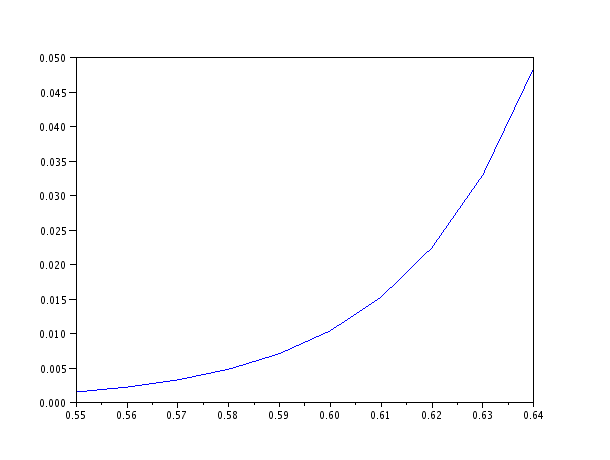
\includegraphics[width=10cm]{II-2.png} \end{center} 
   \end{multicols}
  
  \subsection{Donner le modèle équivalent de la jonction polarisée en direct et calculer les valeurs des composants correspondant à un courant de $7 mA$.}
  Le modèle équivalent de la jonction polarisée en direct est un condensateur $C_d$ en parallèle à une résistance $r_d$, où, pour une jonction $P^+N$, $C_d = \cfrac{I W_n^2}{2 D_p U_T}$ et $r_d = \cfrac{U_T}{I}$.

  AN :$r_d = 3.71 \Omega$ \& $C_d = 6.75\cdot 10^{-10}F$
  
  \subsection{Quelle sera la fréquence maximale d’une tension sinusoïdale petit signal appliquée à la diode polarisée suivant le point précédemment calculé. Quelles modifications structurelles pourriez-vous proposer pour augmenter cette fréquence de coupure ?}
  Comme dans tout filtre passe-bas, $\tau = r_d C_d$, et $f_c = \cfrac{1}{2\pi\tau}$.

  AN : $f_c = 6.34\cdot 10^7Hz$

  Afin que la diode puisse fonctionner à plus haute fréquence, il est possible de diminuer la taille de la diode (mais on réduit alors sa résistance mécanique), ce qui aura pour effet d'augmenter $f_c$.

  On peut aussi diminuer le dopage ou changer de semi-conducteur afin d'augmenter la mobilité des porteurs.

 \section{La diode en redressement}
  \subsection{Ecrire la loi des mailles pour le circuit. En déduire l’expression de $I$, l’intensité du courant dans le circuit en fonction de $E$ et de $U$. Cette équation est celle de la droite de charge statique $\Delta$ du circuit.}
   Loi des mailles : $E = U_R + U$. On en déduit l'expression de $I = \cfrac{U_R}{R} = \cfrac{E-U}{R}$.

  \subsection{Tracer cette droite $\Delta$ sur le graphique tracé au paragraphe précédent et déterminer le point de fonctionnement $P$ du circuit (Intensité traversant le circuit et tension aux bornes de la diode).}

   \begin{center}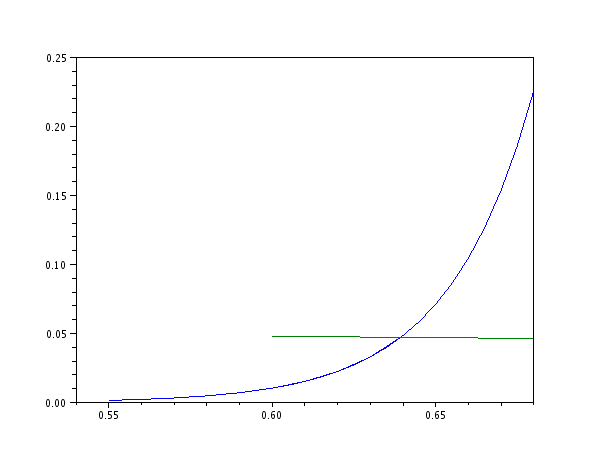
\includegraphics[width=10cm]{III-2.png}\end{center}
  
  \subsection{La densité maximale de courant admise par le silicium est $J_{max} = 300 A\cdot cm^{-2}$. En déduire la puissance maximale $P_{max}$ admissible par la diode.}
  $P=RI^2$, où $R=\cfrac{\rho l}{S} = \cfrac{\rho_n X_n + \rho_p X_p}{A_j}$ et $I=JS$. On a donc $P=(\rho_n X_n + \rho_p X_p) J^2 A_j$. 
  
  Or $\rho_n = \cfrac{1}{q\left(N_D \mu_n + \cfrac{n_i^2}{N_D} \mu_p\right)} \simeq \cfrac{1}{q N_D \mu_n}$ et $\rho_p = \cfrac{1}{q\left(\cfrac{n_i^2}{N_A}\mu_n+N_A \mu_p\right)} \simeq \cfrac{1}{q N_A \mu_p}$

  AN : $P_{MAX} = 422mW$
 
 \section{Fichier Scilab}
  Voici le fichier scilab qui contient toutes nos applications numériques et nos graphes :

  \inputminted[linenos]{matlab}{calculs.sci}
\end{document}
